% ju -- https://bw1.eu -- 27-April-18  -- texDummyPrint.tex
% Modified source from 
% <https://www.dcl.hpi.uni-potsdam.de/media/theses/>
%
\documentclass{scrbook} % <= Druckversion: "scrbook", Bildschirmversion: "scrreprt"
\newcommand\bcor{12mm} % <= Bindungskorrektur fuer Druckversion
\usepackage{content/ju}% meine Einstellung

% ABOUT
\newcommand{\typ}{Projekt}
\newcommand{\autor}{Jan Unger}
\newcommand{\titel}{Haupttitel} % wird per Powershell Script ersetzt
\newcommand{\untertitel}{Mitschrift} 
\newcommand{\ort}{Wuppertal}
\newcommand{\datum}{\today}
\newcommand{\website}{https://bw1.eu}

% DOCUMENT
%\KOMAoption{draft}{true} % <= z.B. zum "Debuggen" der Overfull-Boxes
\bibliography{content/literatur}% meine Literatur
\bibliography{content/literatur-laufen}% meine Literatur

\begin{document}
	\selectlanguage{ngerman}

	% Einband
	\pagenumbering{alph}
	\ifisbook% ju -- https://bw1.eu -- 25-April-18  -- coverpage.tex 
% Modified source from 
% <https://www.dcl.hpi.uni-potsdam.de/media/theses/>
%
\begin{titlepage}
	\setlength{\evensidemargin}{0.5\evensidemargin+0.5\oddsidemargin}
	\setlength{\oddsidemargin}{\evensidemargin}

	\centering
	
	\raisebox{-0.5\height}{
\includegraphics[width=9cm]{content/titelbild-black.pdf}}
	\hspace*{.2\textwidth}
	\raisebox{-0.5\height}{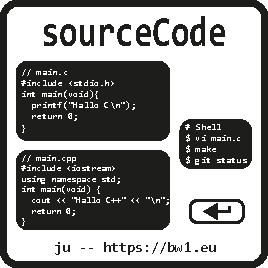
\includegraphics[width=1cm]{content/logo-black.pdf}}

	\vspace*{4\baselineskip}
	{\usekomafont{subject}\typ}\par
	

	{\usekomafont{title}\titel\par}
	\vspace*{\baselineskip}
	{\usekomafont{subtitle}\untertitel}\par

	\vfill

\end{titlepage}

\fi
	\ifisbook\cleardoubleemptypage\fi

	% (Haupt-)Titelseite, Zusammenfassung, ggf. Danksagung & Inhaltsverzeichnis
	\pagenumbering{roman}
	% ju -- https://bw1.eu -- 25-April-18  -- titelpage.tex 
% Modified source from 
% <https://www.dcl.hpi.uni-potsdam.de/media/theses/>
%
\begin{titlepage}
	\setlength{\evensidemargin}{0.5\evensidemargin+0.5\oddsidemargin}
	\setlength{\oddsidemargin}{\evensidemargin}

	\centering
	
	\raisebox{-0.5\height}{
\includegraphics[width=9cm]{content/titelbild.pdf}}
	\hspace*{.2\textwidth}
	\raisebox{-0.5\height}{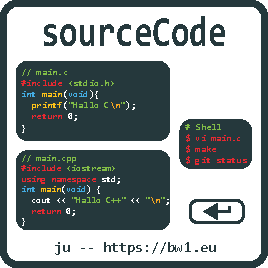
\includegraphics[width=1cm]{content/logo.pdf}}
	\hfill
	\vspace{3mm}
	{\color{meinblue} \rule{\textwidth}{3pt}}
	

	\vspace*{4\baselineskip}
	{\usekomafont{subject}\typ}\par
	
	\vfill
	{\usekomafont{title}\titel\par}
	\vspace*{\baselineskip}
	{\usekomafont{subtitle}\untertitel}\par
	
	\vfill
	{\textbf{\iflanguage{ngerman}{von}{by}}\\ 
		\smallskip\usekomafont{author}\autor}\par
	
	\vfill
	{\usekomafont{date}\ort}\par

	\vspace*{\baselineskip}
	{\usekomafont{date}\datum}\par
  
	\begin{flushleft}
	\vfill
  {\qrcode[hyperlink,height=1.5cm]{\website}}\par
	\end{flushleft}

	\setcounter{page}{1}

\end{titlepage}


	%\ifisbook\cleardoubleemptypage\fi% ju -- https://bw1.eu -- 25-April-18  -- zusammenfassung.tex 
% Modified source from 
% <https://www.dcl.hpi.uni-potsdam.de/media/theses/>
%
% deutsche Zusammenfassung
\null\vfil
\begin{otherlanguage}{ngerman}
\begin{center}\textsf{\textbf{\abstractname}}\end{center}

\noindent Dies hier ist ein Blindtext zum Testen von Textausgaben. Wer diesen Text liest, 
ist selbst schuld. Der Text gibt lediglich den Grauwert der Schrift an. 
Ist das wirklich so? Ist es gleichgültig, ob ich schreibe: "Dies ist ein Blindtext" 
oder "Huardest gefburn"? Kjift - mitnichten! Ein Blindtext bietet mir wichtige Informationen.

\end{otherlanguage}
\vfil\null



% example
	%\ifisbook\cleardoubleemptypage\fi% ju -- https://bw1.eu -- 25-April-18  -- danksagung.tex 
% Modified source from 
% <https://www.dcl.hpi.uni-potsdam.de/media/theses/>
%
\vspace*{\fill}
\begin{center}\textsf{\textbf{Danksagung}}\end{center}

\noindent Dies hier ist ein Blindtext zum Testen von Textausgaben. Wer diesen Text liest, 
ist selbst schuld. Der Text gibt lediglich den Grauwert der Schrift an. 
Ist das wirklich so? Ist es gleichgültig, ob ich schreibe: "Dies ist ein Blindtext" 
oder "Huardest gefburn"? Kjift - mitnichten! Ein Blindtext bietet mir wichtige Informationen.

\vspace*{\fill}% example
	\tableofcontents
	\cleardoublepage

	% Textteil
	\pagenumbering{arabic}
	%\chapter{Kapitel}
	%\include{content/Latex-Spickzettel} % Latex-Spickzettel

	% Inhalt 
% ju -- https://bw1.eu -- 11-Okt-18
\chapter{Kapitel} 
\input{tex/Abbildungen}

\chapter{Kapitel} 
\input{tex/Inhalt}

\chapter{Kapitel} 
\input{tex/Links}

\chapter{Kapitel} 
\input{tex/Python-Notiz}

\chapter{Kapitel} 
\input{tex/Quellcode}

 % wird per Powershell Script ersetzt

	% ggf. Anhang
	%\appendix% ju -- https://bw1.eu -- 25-April-18  -- anhang.tex 
% Modified source from 
% <https://www.dcl.hpi.uni-potsdam.de/media/theses/>
%
\chapter{\appendixname}

\section{Eins}
Auch gibt es niemanden, der den Schmerz an sich liebt, sucht oder wünscht, nur, weil er Schmerz ist, es sei denn, es kommt zu zufälligen Umständen, in denen Mühen und Schmerz ihm große Freude bereiten können. Um ein triviales Beispiel zu nehmen, wer von uns unterzieht sich je anstrengender körperlicher Betätigung, außer um Vorteile daraus zu ziehen? Aber wer hat irgend ein Recht, einen Menschen zu tadeln, der die Entscheidung trifft, eine Freude zu genießen, die keine unangenehmen Folgen hat, oder einen, der Schmerz vermeidet, welcher keine daraus resultierende Freude nach sich zieht? Auch gibt es niemanden, der den Schmerz an sich liebt, sucht oder wünscht, nur, weil er Schmerz ist, es sei denn, es kommt zu zufälligen Umständen, in denen Mühen und Schmerz ihm große Freude bereiten können. Um ein triviales Beispiel zu nehmen, wer von uns unterzieht sich je anstrengender körperlicher Betätigung, außer um Vorteile daraus zu ziehen? Aber wer hat irgend ein Recht, einen Menschen zu tadeln, der die Entscheidung trifft, eine Freude zu genießen, die keine unangenehmen Folgen hat, oder einen, der Schmerz vermeidet, welcher keine daraus resultierende Freude nach sich zieht?Auch gibt es niemanden, der den Schmerz an sich liebt, sucht oder wünscht, nur,

\section{Zwei}
Auch gibt es niemanden, der den Schmerz an sich liebt, sucht oder wünscht, nur, weil er Schmerz ist, es sei denn, es kommt zu zufälligen Umständen, in denen Mühen und Schmerz ihm große Freude bereiten können. Um ein triviales Beispiel zu nehmen, wer von uns unterzieht sich je anstrengender körperlicher Betätigung, außer um Vorteile daraus zu ziehen? Aber wer hat irgend ein Recht, einen Menschen zu tadeln, der die Entscheidung trifft, eine Freude zu genießen, die keine unangenehmen Folgen hat, oder einen, der Schmerz vermeidet, welcher keine daraus resultierende Freude nach sich zieht? Auch gibt es niemanden, der den Schmerz an sich liebt, sucht oder wünscht, nur, weil er Schmerz ist, es sei denn, es kommt zu zufälligen Umständen, in denen Mühen und Schmerz ihm große Freude bereiten können. Um ein triviales Beispiel zu nehmen, wer von uns unterzieht sich je anstrengender körperlicher Betätigung, außer um Vorteile daraus zu ziehen? Aber wer hat irgend ein Recht, einen Menschen zu tadeln, der die Entscheidung trifft, eine Freude zu genießen, die keine unangenehmen Folgen hat, oder einen, der Schmerz vermeidet, welcher keine daraus resultierende Freude nach sich zieht?Auch gibt es niemanden, der den Schmerz an sich liebt, sucht oder wünscht, nur,

\section*{Drei (ohne extra Eintrag im Inhaltsverzeichnis)}
Auch gibt es niemanden, der den Schmerz an sich liebt, sucht oder wünscht, nur, weil er Schmerz ist, 

\section*{Vier (ohne extra Eintrag im Inhaltsverzeichnis)}
Auch gibt es niemanden, der den Schmerz an sich liebt, sucht oder wünscht, nur, weil er Schmerz ist,  % example

	% Bibliographie
	\ifisbook\cleardoubleemptypage\fi
	\phantomsection\addcontentsline{toc}{chapter}{\refname}
	\printbibliography[category=cited]

	% Eigenstaendigkeitserklaerung
	%\ifisbook\pagestyle{plain}\cleardoubleemptypage% ju -- https://bw1.eu -- 25-April-18  -- erklaerung.tex 
% Modified source from 
% <https://www.dcl.hpi.uni-potsdam.de/media/theses/>
%
\begin{otherlanguage}{ngerman}

\begin{center}\textsf{\textbf{Eidesstattliche Erklärung}}\end{center}
Hiermit versichere ich, dass meine Arbeit \enquote{\titel} selbständig verfasst wurde und dass keine anderen Quellen und Hilfsmittel als die angegebenen benutzt wurden. Diese Aussage trifft auch für alle Implementierungen und Dokumentationen im Rahmen dieses Projektes zu.\\

\noindent
\ort, den \datum,
\vspace{2cm}

\begin{center}
\begin{tabular}{C{6cm}}
\hline
{\small({\autor})}
\end{tabular}
\end{center}

\end{otherlanguage}


\fi % example

\end{document}
%============================
%============================
%============================